% ============================================================================================
% This is a LaTeX template used for the course
%
%  I M A G E   B A S E D   B I O M E T R I C S
%
% Faculty of Computer and Information Science
% University of Ljubljana
% Slovenia, EU
%
% You can use this template for whatever reason you like.
% If you have any questions feel free to contact
% ziga.emersic@fri.uni-lj.si
% ============================================================================================

\documentclass[9pt]{IEEEtran}

% basic
\usepackage[english]{babel}
\usepackage{graphicx,epstopdf,fancyhdr,amsmath,amsthm,amssymb,url,array,textcomp,svg,listings,hyperref,xcolor,colortbl,float,gensymb,longtable,supertabular,multicol,placeins}

 % `sumniki' in names
\usepackage[utf8x]{inputenc}

 % search and copy for `sumniki'
\usepackage[T1]{fontenc}
\usepackage{lmodern}
\input{glyphtounicode}
\pdfgentounicode=1

% tidy figures
\graphicspath{{./figures/}}
\DeclareGraphicsExtensions{.pdf,.png,.jpg,.eps}

% correct bad hyphenation here
\hyphenation{op-tical net-works semi-conduc-tor trig-gs}

\usepackage{float}

% ============================================================================================

\title{\vspace{0ex} %
% TITLE IN HERE:
Ear Detection
\\ \large{Assignment \#2}\\ \normalsize{Image Based Biometrics 2020/21, Faculty of Computer and Information Science, University of Ljubljana}}
\author{ %
% AUTHOR IN HERE:
Dimitar~Stefanov
\vspace{-4.0ex}
}

% ============================================================================================

\begin{document}

\maketitle

\section{Introduction}
I started working on Assignment 2 by testing out Haar cascades for ear detection on images from the Annotated Web Ears Dataset. I obtained these cascades from Github. I also came across a couple of LBP detectors, so I decided to include one in the \href{https://github.com/dstefanov46/IBB_Assignment2}{code} I submitted in addition to this report. To improve the scores of these detectors, I used the cascade "haarcascade\_frontalface\_default.xml" that comes along with the OpenCV package. This is a well made cascade, and therefore I believed it would be able to do satisfactory face detection on my test set. This could in turn help me perform better ear detection as my ear cascades would only focus on the face region detected previously by the face detection cascade. So, as a final step, I merged the 3 ear detectors and the face detector hoping to get the most optimal detection.

\section{Results}
During the laboratory tutorials, it was elaborated on multiple occasions why the metric, which presents the performance of the detector in a most realistic fashion, is Intersection over Union. Therefore, without further doubt, I decided to use this measure as an indicator of how well my detectors work. The results for the initial versions of the 3 ear detectors are presented below:

\begin{figure}[H]
    \centering
    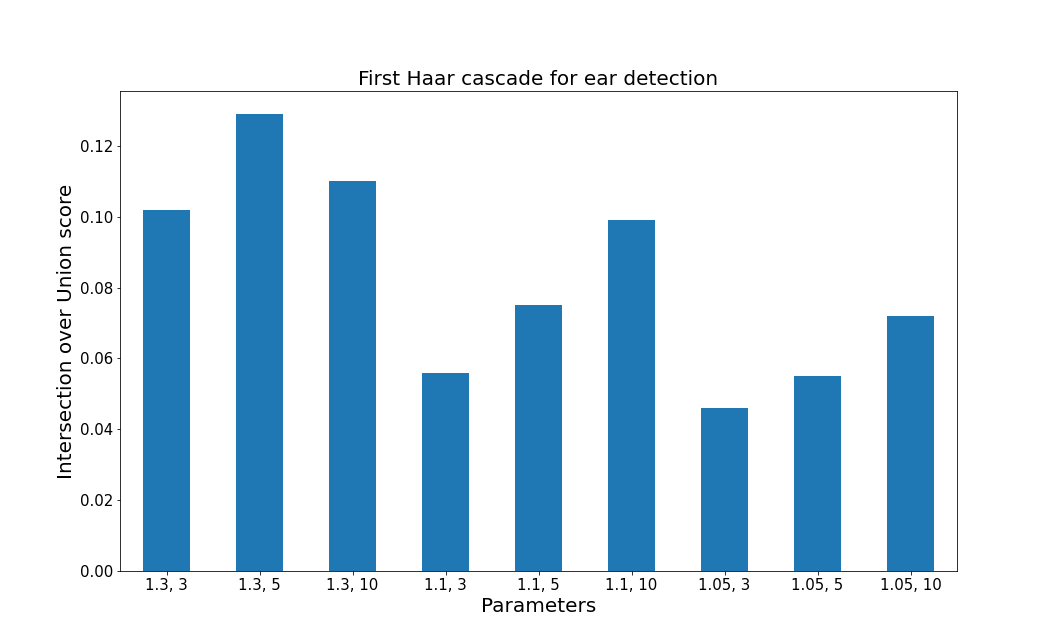
\includegraphics[width=1\columnwidth]{plot_1.1}
    \label{fig:plot_1.1}
\end{figure}

\begin{figure}[H]
    \centering
    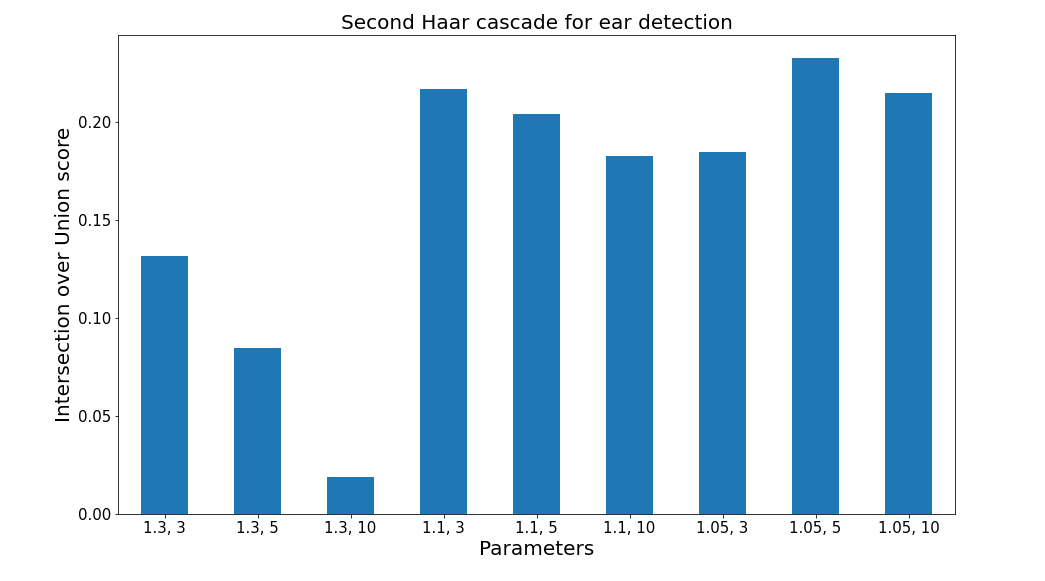
\includegraphics[width=1\columnwidth]{plot_1.2}
    \label{fig:plot_1.2}
\end{figure}

\begin{figure}[H]
    \centering
    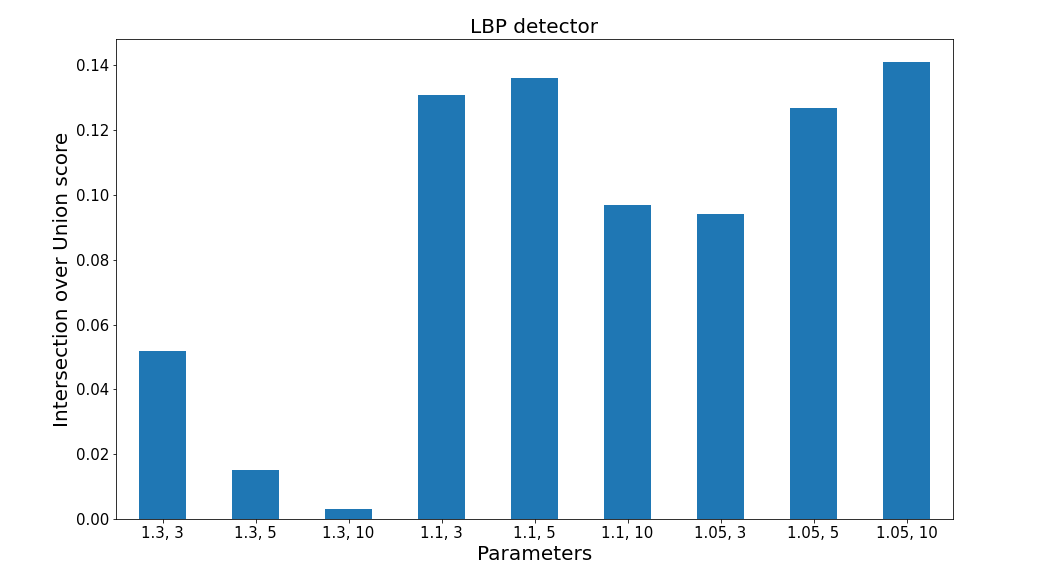
\includegraphics[width=1\columnwidth]{plot_1.3}
    \caption{The three barplots show the Intersection over Union scores of our two Haar ear cascades and the LBP detector. In the figure, we can observe how changing of parameters impacts the performance of the detectors.}
    \label{fig:plot_1.3}
\end{figure}

As we can see, the detectors do not perform extremely well. I tried various scale factors as well as various minNeighbours values. The minNeighbours parameter is usually set to be a number between 3 and 6, but here we took also 10 into consideration. This was due to the fact that our detectors detected a lot of false positives, and in order to resolve this problem, as general practice, you increase the minNeighbours parameter. Unfortunately, even a higher value for the minNeighbours parameter didn't improve the performance of the detectors significantly. The reasons for this can be a lot, ranging from the fact that Viola-Jones detectors simply cannot produce very high results as a CNN could for instance, to the fact that our cascades have probably been trained on quite different pictures than the ones on which they are tested. 

As a second idea to boost the scores of the cascades, I decided to use a face detector and ear detector together. To be more precise, if the ear cascade labels some part of the picture as ear, and that section is not inside the face region detected by the face detector, then we shouldn't consider those pixels as part of an ear. That way, I hoped to get rid of some of the inaccuracies of my ear detectors. Nevertheless, this new method brought the opposite effect as it is depicted in Figure 2.

This poor performance comes as a result of our Haar face cascade capturing only the face of a person, and rarely some other parts of the head. Subsequently, the intersection between the face region detected by the face cascade and the ear region detected by one of the ear cascades is rather low. And, by not taking into account that ear region, which is not in the intersection, when calculating the intersection over union we get an even worse score. In order to resolve this problem, we tried two other face cascades already added to the OpenCV package: "haarcascade\_profileface.xml" and "lbpcascade\_profileface.xml". Nevertheless, as the first face detector, these detectors also didn't include a person's ears in the face region in most images, and in a great deal of images struggled to even locate the face.

\begin{figure}[h]
    \centering
    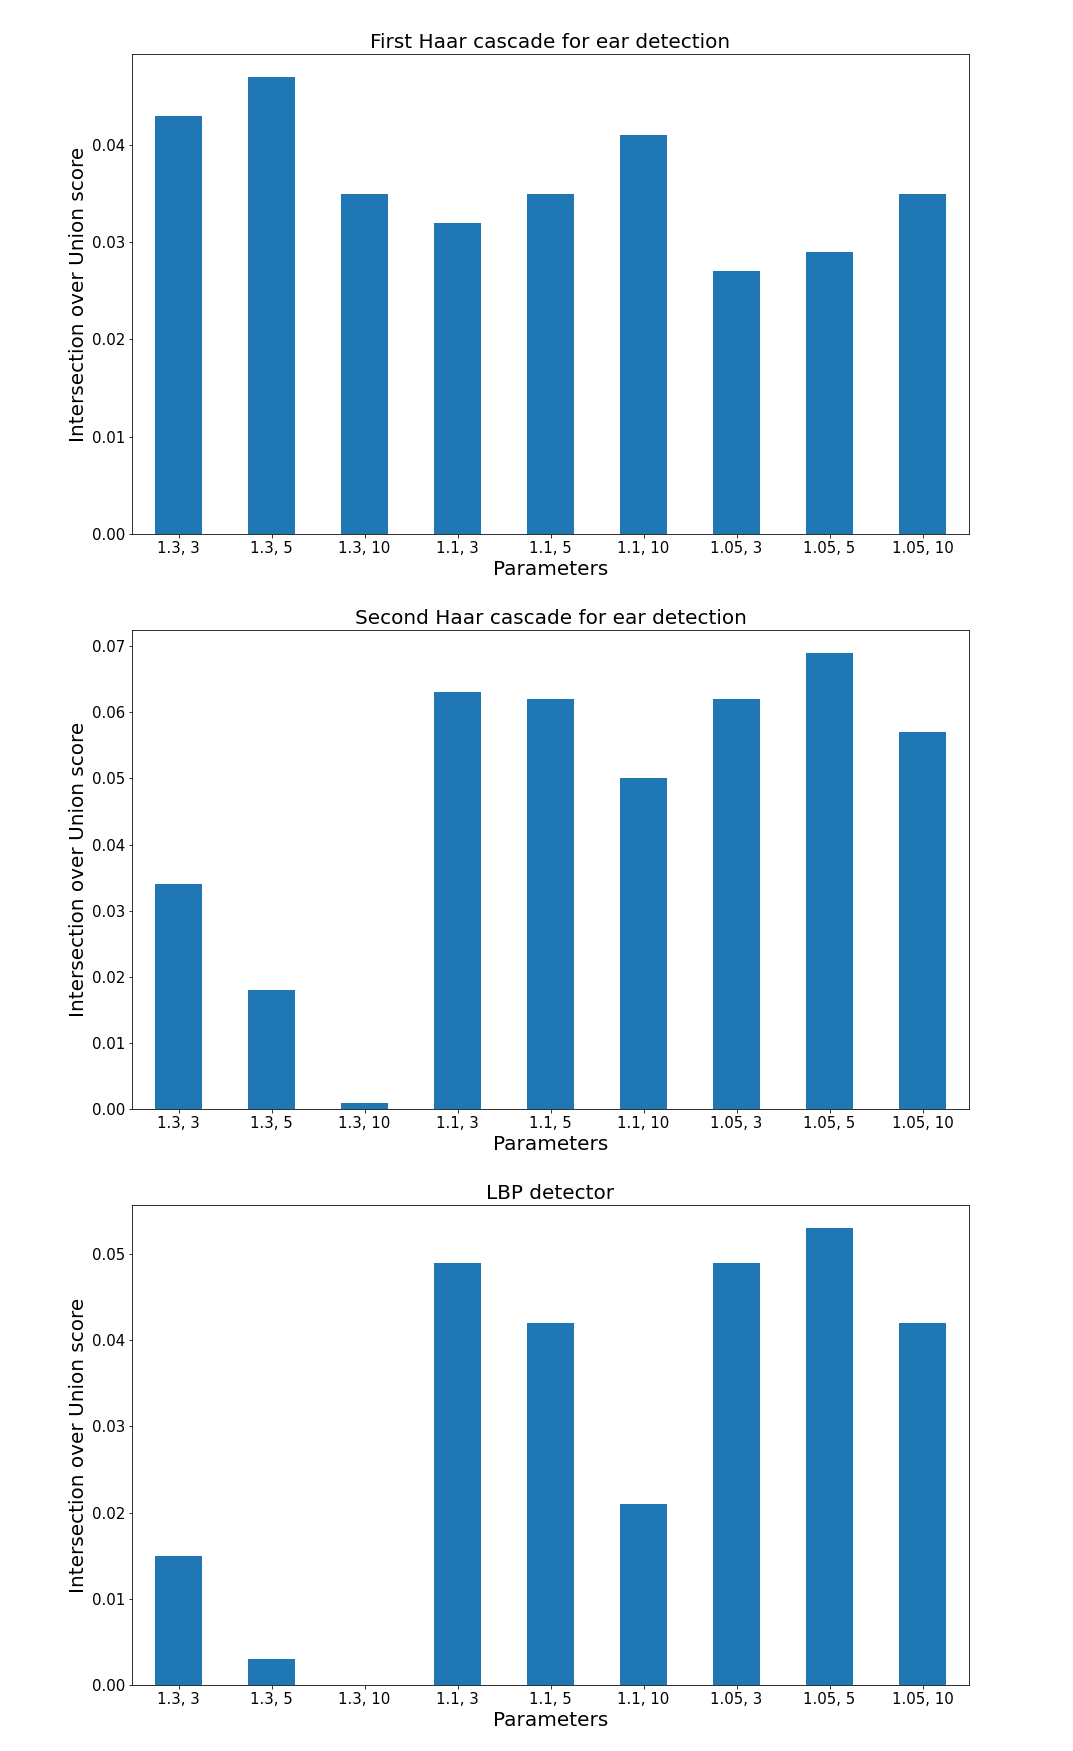
\includegraphics[width=1\columnwidth]{plot_2.2}
    \caption{The figure presents the Intersection over Union scores of combinations of face and ear detector. The parameters of the ear detectors are the same as in Figure 1, however there's a decrease in their performance.}
    \label{fig:plot_2.2}
\end{figure}

\section{Conclusion}
To sum up, we didn't manage to achieve very high scores with our detectors in spite of optimizing their parameters. The idea of combining them with a face detector sounded promising, but because the face cascades couldn't capture a significant part of the ear region in the pictures, their addition to our model turned out to be unhelpful. 

Perhaps, we might get different, better performance results if the detectors are tested against a different set of photos. So, that's certainly one idea to explore. However, if we would like to have top-notch results, then instead of a Haar cascade we should opt for a convolutional neural network.

\bibliographystyle{IEEEtran}
\begin{thebibliography}{99}
\bibitem{book1} OpenCV. Face Detection using Haar Cascades. \url{https://opencv-python-tutroals.readthedocs.io/en/latest/py_tutorials/py_objdetect/py_face_detection/py_face_detection.html}, 2013.
\bibitem{book2} shivangbansal. Haar-Cascade-Ear-Training. \url{https://github.com/shivangbansal/Haar-Cascade-Ear-Training}, Feb 3, 2018.
\bibitem{book3} atduskgreg. opencv-processing. \url{https://github.com/atduskgreg/opencv-processing/tree/master/lib/cascade-files}, Jul 17, 2013.
\bibitem{book4} Computer Vision Laboratory, Faculty of Computer and Information Science, University of Ljubljana. Annotated Web Ears Dataset - AWE Dataset. \url{http://awe.fri.uni-lj.si/}, 2017.
\end{thebibliography}

*The URL of my Github repository containing the code written to obtain the above presented results is the following: \url{https://github.com/dstefanov46/IBB_Assignment2}.
\end{document}